%!TEX TS-program = xelatex
%!TEX encoding = UTF-8 Unicode
\documentclass[10pt]{article}      
\usepackage[usenames,dvipsnames]{xcolor}
\usepackage{geometry}
%!TEX root = CurriculumVitae.tex
\usepackage{graphicx}
\usepackage{amsmath}
\usepackage{epstopdf}
\usepackage{datetime}
\usepackage{enumerate}
\usepackage{wrapfig}
\usepackage{graphicx}
\usepackage{amssymb}
\newtimeformat{dottime}{\twodigit{\THEHOUR}:\twodigit{\THEMINUTE}}
\settimeformat{ampmtime}
\usepackage[margin=1pt,font=small,labelfont=bf]{caption}
\usepackage{fancyhdr}
\usepackage{xhfill}
\usepackage[inline]{enumitem}
\usepackage{soul}
\usepackage{scrextend}
\usepackage{lastpage}
\usepackage[usenames,dvipsnames]{xcolor}
\usepackage{etoolbox}
\usepackage{tikz}
\usepackage{sectsty}
\sectionfont{\normalsize}
\def\thesection{Section \alph{section}: \hspace{-12pt}}

\newrobustcmd*{\mytriangle}[2]{\tikz{\filldraw[draw=#1,fill=#1,rotate=#2] (0,0) --
(0.2cm,0) -- (0.1cm,0.2cm);}}

\newrobustcmd*{\mysquare}[2]{\tikz{\filldraw[draw=#1,fill=#1,rotate=#2] (0,0) --
(0.2cm,0) -- (0.2cm,0.2cm) -- (0.0cm,0.2cm);}}

\newrobustcmd*{\mytriangleb}{\tikz{\filldraw[draw=Black,fill=Black,rotate=-90] (0,0) --
(0.2cm,0) -- (0.1cm,0.2cm);}~}

\newrobustcmd*{\mytriangleg}{\tikz{\filldraw[draw=OliveGreen,fill=ForestGreen,rotate=-90] (0,0) --
(0.2cm,0) -- (0.1cm,0.2cm);}~}

\newcommand{\mycircle}[2][OrangeRed,fill=OrangeRed]{\tikz[baseline=-0.5ex]\draw[#1,fill=#1,radius=#2] (0,0) circle ;}%

\newcommand{\raisedrule}[2][1em]{\leaders\hbox{\rule[#1]{1pt}{#2}}\hfill}

\setlength{\parindent}{0pt}

%\usepackage{hyperref}
%\hypersetup{colorlinks=false,citecolor=cyan,linkcolor=black,linktocpage=true}
        
\renewcommand{\refname}{}
\newcounter{mycounter}  
\newenvironment{enumeratenew}
 {\begin{list}{~}{\usecounter{mycounter} \labelsep=0em \labelwidth=5pt \leftmargin=0pt \itemindent=5pt}}
 {\end{list}}

\definecolor{MyGray}{rgb}{0.95,0.95,0.975}

\definecolor{mycolor}{rgb}{0.02, 0.435, 0.698}


%%%%%%%%%%%%%%%%%%%%%%%%%%%%%%%%%%%%%%%%%%%%%%%%%%%%%%%%%%%%%% 
\newcommand{\subtitle}[1]{
{\mysquare{BrickRed}{-90}~~\textbf{\textcolor{BrickRed}{\large #1 ~}}}\xrfill[0pt]{2pt}[BrickRed]\\%{\color{OrangeRed}\hrulefill}\\ 
%\mytriangle{BrickRed}{-90}~
%{\textbf{\textcolor{BrickRed}{{\large #1}}}}  \\[-5pt]\noindent
}
%%%%%%%%%%%%%%%%%%%%%%%%%%%%%%%%%%%%%%%%%%%%%%%%%%%%%%%%%%%%%% 
\newcommand{\subtitlea}[2]{
%{\mytriangle{OrangeRed}{-90}~\textbf{\textcolor{NavyBlue}{#1}}}~\mytriangle{OrangeRed}{90}\xrfill[2pt]{1.5pt}[OrangeRed]\\%{\color{OrangeRed}\hrulefill}\\ \mytriangle{BrickRed}{-90}~
{\mysquare{BrickRed}{-90}~~\textbf{\textcolor{BrickRed}{\large #1 ~}}}\xrfill[0pt]{2pt}[BrickRed]\\[-5pt]
\begin{addmargin}[1em]{0em}
#2
\end{addmargin}
\vspace{10pt}
}
%%%%%%%%%%%%%%%%%%%%%%%%%%%%%%%%%%%%%%%%%%%%%%%%%%%%%%%%%%%%%%%%%%%%%%%%
\newenvironment{tightcenter}{%
  \setlength\topsep{0pt}
  \setlength\parskip{0pt}
  \begin{center}
}{%
  \end{center}
}
%%%%%%%%%%%%%%%%%%%%%%%%%%%%%%%%%%%%%%%%%%%%%%%%%%%%%%%%%%%%%% 
\newenvironment{list3}{
\vspace{-0.4in}
  \begin{enumerate}{%
      \setlength{\itemsep}{-0.2in}
      \setlength{\parsep}{-0.2in} \setlength{\parskip}{0in}
      \setlength{\topsep}{0in} \setlength{\partopsep}{0in} 
      \setlength{\leftmargin}{-0.8in}}}{\end{enumerate}}
%%%%%%%%%%%%%%%%%%%%%%%%%%%%%%%%%%%%%%%%%%%%%%%%%%%%%%%%%%%%%%       

\usepackage[firstinits=true,backend=bibtex,style=authoryear,sorting=none,maxbibnames=99,maxnames=15]{biblatex}
 
\renewbibmacro{in:}{}

\DeclareFieldFormat{journaltitle}{\textit{#1}}
\DeclareFieldFormat[article,book,proceedings,inbook,incollection,inproceedings,patent,thesis,unpublished]{title}{\textit{\textcolor{Black}{#1}}}
\DeclareFieldFormat
  [article,inbook,incollection,proceedings,inproceedings,patent,thesis,unpublished]
  {title}{\mkbibquote{\textcolor{Black}{\bf \textit{#1}}\isdot}}
\AtEveryBibitem{
%\clearfield{year}
\clearfield{volume}
\clearfield{number}
\clearfield{pages}
}
\DeclareFieldFormat{labelnumberwidth}{\mytriangle{Black}{-90}}
\defbibenvironment{bibliography}
  {\list
     {\printtext[labelnumberwidth]{%
        \printfield{prefixnumber}%
        \printfield{labelnumber}}}
     {\setlength{\labelwidth}{\labelnumberwidth}%
      \setlength{\leftmargin}{20pt}%
      \setlength{\labelsep}{2pt}%
      \addtolength{\leftmargin}{\labelsep}% 
      \setlength{\itemsep}{\bibitemsep}%
      \setlength\bibhang{10pt}
      \setlength{\parsep}{\bibparsep}}%
      \renewcommand*{\makelabel}[1]{\hss##1}}
  {\endlist}
  {\item}

\addbibresource{~/Dropbox/Public/CollectedPapers/MasterBibliography.bib}

\fancypagestyle{rest}
{      
\fancyhead[L]{}
\fancyhead[R]{}
\fancyhead[C]{}
\fancyfoot[C]{[\thepage]}
\fancyfoot[R]{\tiny \color{Gray}Last Modified \today}
}
\setlength{\footskip}{0.5cm}
\setlength{\voffset}{0.0cm} 
\setlength{\headheight}{-6pt} 
\renewcommand{\headrulewidth}{0.0pt}
\renewcommand{\footrulewidth}{0.0pt}

   

\usepackage{fontspec}
\usepackage{tcolorbox}
\definecolor{mygray}{rgb}{0.2,0.2,0.2}% Rule colour
\usepackage{etaremune}
\usepackage[colorlinks=true,
            linkcolor=gray,
            urlcolor=black,
            citecolor=gray]{hyperref}
            
\setlist[description]{%
  font={\color{mygray}}, % set the label font
}
\definecolor{harvard}{rgb}{0.788,0,0.086}
\definecolor{ivy}{RGB}{78,136,199}
  \geometry{a4paper,left=18mm,top=15mm,headsep=2\baselineskip,right=18mm,textheight=63\baselineskip,headheight=5\baselineskip}
          
\begin{document}

\baselineskip15pt
\setlength{\parskip}{0pt}
%%%%%%%%%%%%%%%%%%%%%%%%%%%%%%%%%%%%%%%%%%%%%%%%%%%%%%%%%%%%%%%%%%%%%%%%
\setmainfont[Mapping=tex-text]{Roboto Light}
\pagestyle{rest}
\setcounter{page}{1}
\setcounter{section}{1}
\hfill {\Large \color{harvard}\LARGE \textbf{Harsha}} {\Large \color{harvard}\LARGE {Suresh}} {\Large \color{harvard}\LARGE \textbf{Bhat}} \\[-15pt]

\hfill \textit{Chargé de Recherche de Classe Normale, CNRS}\\[-15pt]

\hfill \textit{École Normale Supérieure, Paris}\\[-15pt]

\hfill \textit{Laboratoire de Géologie, 24 Rue Lhomond, 75005, Paris, France}\\[1.5cm]
%%%%%%%%%%%%%%%%%%%%%%%%%%%%%%%%%%%%%%%%%%%%%%%%%%%%%%%%%%%%%%%%%%%%%%%%
\subtitlea{PERSONAL INFORMATION}{
 Email: \url{harsha.bhat@ens.fr}~~~~Nationality: Indian~~~~Website: \url{https://harshasbhat.github.io}
}
%%%%%%%%%%%%%%%%%%%%%%%%%%%%%%%%%%%%%%%%%%%%%%%%%%%%%%%%%%%%%%%%%%%%%%%%
\subtitlea{EDUCATION}{
\vspace{8pt}
\noindent\begin{tabular*}{\textwidth}{@{}l|c|c|r} 
{\it École Normale Supérieure, France} & { H. D. R.} & {\it Supershear Earthquakes} & {2021/01} \\[3pt]
{\it Harvard University, USA} & { Ph. D.} & {\it Mechanical Sciences} & {2007/06} \\[3pt]
{\it Harvard University, USA} & { M. S.} & {\it Engineering Sciences} & {2002/06} \\[3pt] 
{\it NITK, India} & { B. E.} & {\it Civil Engineering} & {2001/06}
\end{tabular*}
}
%%%%%%%%%%%%%%%%%%%%%%%%%%%%%%%%%%%%%%%%%%%%%%%%%%%%%%%%%%%%%%%%%%%%%%%%%
\subtitlea{CURRENT POSITION}{
\vspace{8pt}
\noindent\begin{tabular}{@{}l | l | l}
{\it  École Normale Supérieure, France} & {2016/05~\mytriangle{Black}{-90}} Present&
\it CNRS Research Scientist \\[4pt]
{\it  California Institute of Technology, USA} & {2018/12~\mytriangle{Black}{-90}} Present&
\it Visiting Professor in Aeronautics
\end{tabular}
}
%%%%%%%%%%%%%%%%%%%%%%%%%%%%%%%%%%%%%%%%%%%%%%%%%%%%%%%%%%%%%%%%%%%%%%%%%
\subtitlea{PAST POSITIONS}{
\vspace{8pt}
\noindent\begin{tabular}{@{}l | l | l}
{\it  Institut de Physique du Globe de Paris, France} & {2012/01~\mytriangle{Black}{-90}~2016/05}&
\it CNRS Research Scientist \\[4pt]
{\it  University of Southern California, USA} & {2010/03~\mytriangle{Black}{-90}~2011/12}&
\it Asst. Professor (Research)  \\[4pt]
{\it  University of Southern California, USA} & {2007/11~\mytriangle{Black}{-90}~2010/03}&
\it Post Doctoral Fellow  \\[4pt]
{\it  California Institute of Technology, USA} & {2007/11~\mytriangle{Black}{-90}~2010/03}&
\it Visitor in Aeronautics \\[4pt]
{\it  Harvard University, USA} & {2007/05~\mytriangle{Black}{-90}~2007/10}&
\it Post Doctoral Fellow \\[4pt]
{\it  Harvard University, USA} & {2001/11~\mytriangle{Black}{-90}~2007/05}&
\it Grad. Research Associate
\end{tabular}
}
\vspace{12pt}
%%%%%%%%%%%%%%%%%%%%%%%%%%%%%%%%%%%%%%%%%%%%%%%%%%%%%%%%%%%%%%%harvard%%%%%%%%%%%%%
\subtitlea{FUNDING \& GRANTS}{ 
2017-2017~\mytriangle{Black}{-90} 6k€ TelluS INSU - action ALEAS\\
2018-2018~\mytriangle{Black}{-90} 25k€ ENS Actions Incitatives\\
2021-2025~\mytriangle{Black}{-90} 2M€ ERC Consolidator Grant, PERSISMO (Grant No. 865411)
}
%%%%%%%%%%%%%%%%%%%%%%%%%%%%%%%%%%%%%%%%%%%%%%%%%%%%%%%%%%%%%%%%%%%%%%%%%
\subtitlea{HONORS AND AWARDS}{ 
 2018 CNRS Award for Doctoral Supervision and Research\\
 2018 Grand Prix Michel Gouilloud Schlumberger, French Academy of Sciences\\
 2003, 2004 \& 2006 Harvard University Certificate of Distinction in Teaching 
}
%%%%%%%%%%%%%%%%%%%%%%%%%%%%%%%%%%%%%%%%%%%%%%%%%%%%%%%%%%%%%%%%%%%%%%%%%%%%
\subtitlea{TEACHING ACTIVITIES$\dagger$}{
\begin{enumerate*}[label=\textit{\arabic*)}]
\item Mecanique des Milieux Continus \item Active Faults : Geometry \item Seismic Ruptures and Scaling Laws \item  Introduction to Rock Physics \item Mathematical Methods in the Sciences \item Environmental Risks and Disasters \item Ordinary and Partial Differential Equations \item Complex and Fourier Analysis \item Computational Solid and Structural Mechanics \item Solid Mechanics \item Introduction to the Mechanics of Solids \item Mechanics of Fracture  \item  Advanced Geomechanics 
\end{enumerate*}}
{\it \hfill $\dagger$ Classes taught with various colleagues at Harvard, Caltech, IPGP and ENS}\\[20pt]
%%%%%%%%%%%%%%%%%%%%%%%%%%%%%%%%%%%%%%%%%%%%%%%%%%%%%%%%%%%%%%%%%%%%%%%%%
\subtitlea{ORGANISATION OF SCIENTIFIC MEETINGS}{
 June 2019: Coupled Processes In Fracture Propagation In Geo-Materials: From Hydraulic Fractures To Earthquakes: CISM Advanced School, Udine, Italy\\
 April 2015: Seismological Society of America, Multiscale Modeling and Characterization of Fragmentation and Damage Patterns in Fault Zones\\
 December 2014: American Geophysical Union, Fault Zone Properties And Processes During Dynamic Ruptures
}
%%%%%%%%%%%%%%%%%%%%%%%%%%%%%%%%%%%%%%%%%%%%%%%%%%%%%%%%%%%%%%%%%%%%%%%%%
\subtitlea{INSTITUTIONAL RESPONSIBILITIES}{
 2018 Onwards: Team Leader of Faults \& Earthquakes Group, ENS {(\it11 Researchers, 8 postdocs and 8 PhD students)}\\[2pt]
 2018-2019: Co-organizer of the Internal Seminar, ENS
}
%%%%%%%%%%%%%%%%%%%%%%%%%%%%%%%%%%%%%%%%%%%%%%%%%%%%%%%%%%%%%%%%%%%%%%%%%
%\subtitlea{LANGUAGES}{
%English -- {\it Native} ~|~ French -- {\it Conversant} ~|~ Hindi -- {\it Fluent} ~|~ Kannada -- {\it Native} ~|~ Tulu -- {\it Native} ~|~ Havyaka -- {\it Native} ~|~ Sanskrit -- {\it Moderate} ~|~ Konkani -- {\it Moderate} ~|~ Bengali -- {\it Basic}     
%}
%%%%%%%%%%%%%%%%%%%%%%%%%%%%%%%%%%%%%%%%%%%%%%%%%%%%%%%%%%%%%%%%%%%%%%%%%
\subtitle{BOOKS}
\vspace{-15pt}
\begin{refsegment}
\nocite{thomas2017a,bizzarri2012}
\setlength\bibitemsep{10pt}
\printbibliography[segment=1, title={}, heading=none]
\end{refsegment}
\vspace{15pt}
%%%%%%%%%%%%%%%%%%%%%%%%%%%%%%%%%%%%%%%%%%%%%%%%%%%%%%%%%%%%%%%%%%%%%%%%%
\subtitlea{REVIEWING ACTIVITIES }{
American Geophysical Union
\hspace{10pt} Seismological Society of America
\hspace{10pt} International Journal of Fracture
\hspace{10pt} Geological Society of America
\hspace{10pt} Science
\hspace{10pt} Nature
\hspace{10pt} Journal of the Mechanics and Physics of Solids
\hspace{10pt} European Journal of Mechanics - A/Solids
\hspace{10pt} Earth and Planetary Science Letters
\hspace{10pt} Geophysical Research Letters
\hspace{10pt} Journal of Structural Geology
\hspace{10pt} Proceedings of the National Academies of Science, USA
\hspace{10pt} Geology
\hspace{10pt} Geophysical Journal International
\hspace{10pt} Journal of Applied Mechanics
\hspace{10pt} National Science Foundation
\hspace{10pt} European Research Council
}
%%%%%%%%%%%%%%%%%%%%%%%%%%%%%%%%%%%%%%%%%%%%%%%%%%%%%%%%%%%%%%%%%%%%%%%%%
%\subtitlea{MEMBERSHIPS OF SCIENTIFIC SOCIETIES}{
% American Geophysical Union\\[2pt]
% European Geophysical Union
%}
%%%%%%%%%%%%%%%%%%%%%%%%%%%%%%%%%%%%%%%%%%%%%%%%%%%%%%%%%%%%%%%%%%%%%%%%%
\subtitlea{STUDENTS \& POSTDOCS}{\vspace{0.1cm}
%%%%%%%%%%%%%%%%%%%%%%%%%%%%%%%%%%%%%%%%%%%%%%%%%%%%%%%%%%%%%%%%%%%%%%%%%
\hfill \textbf{\color{harvard} ~\textit{\ul{Undergraduate Students : 6 weeks long research internship}}}\\[-1pt]
\setlist{nolistsep}
\begin{description}[labelindent=0pt ,labelwidth=2cm, labelsep*=2pt, itemsep=4pt,leftmargin =!, style = standard]%
\item[• Phillipe Danre (2017)] Étude de l’impact des marées sur le glissement sismique et asismique des failles actives \textit{(Co-advised with Dr. R. Jolivet, ENS)}
\item[• Hugo Lestrelin (2019)] Theoretical investigation of radiation from a size distribution of fractures\textit{(Co-advised with Dr. L. Bruhat, ENS)}
\item[• Roxane Ferry (2019)] Understanding the relationship between Slow Slip accélérations observed in natural and synthetic GPS \textit{(Co-advised with Dr. J. Jara, ENS)}\\[5pt]\end{description}
%%%%%%%%%%%%%%%%%%%%%%%%%%%%%%%%%%%%%%%%%%%%%%%%%%%%%%%%%%%%%%%%%%%%%%%%%%%%
\hfill \textbf{\color{harvard} ~\textit{\ul{Masters Students : 4-6 month long research internship}}}\\[-1pt]
\setlist{nolistsep}
\begin{description}[labelindent=0pt ,labelwidth=2cm, labelsep*=2pt, itemsep=4pt, leftmargin =!, style = standard]%
\item[• Sonia Fliss (2003)] Fault branching and rupture directivity \textit{(Co-advised with Prof. J. R. Rice \& Dr. R. Dmowska, Harvard)}
\item[• Marion Olives (2004)] Finite fault branches and rupture dynamics: Is it time to look more carefully at fault maps? \textit{(Co-advised with Prof. J. R. Rice \& Dr. R. Dmowska, Harvard)}
\item[• Aurelie Baudet (2004)] Finite element modeling of laboratory experiments on impact and shear rupture of pre-faulted specimens \textit{(Co-advised with Prof. J. R. Rice \& Dr. E. L. Templeton, Harvard)}
\item[• Lucile Bruhat (2012)] Near-field radiation from stopping ruptures \textit{(Co-advised with Prof. J.-P. Vilotte, IPGP)}
\item[• Thibaut Perol (2013)] Micromechanics Based Permeability Evolution In Brittle Materials At High Strain Rates
\item[• Kurama Okubo (2014)] The effect of waste water injection on earthquake nucleation in damaged fault zones
\item[• Victor Barolle (2015)] Metastable phase transformation in the mantle: Evolution of a spinel inclusion into olivine 
\item[• Eleni Kolokytha (2015)] Understanding the role of temperature evolution in the frictional behavior of fault zone and its effect on the seismic cycle \textit{(Co-advised with Dr. M. Y. Thomas)}
\item[• Luc Illien (2018)] Multiseismic phase characterization in laboratory rock deformation experiments, a Numerical and Experimental study \textit{(Co-advised with Dr. N. Brantut)}
\item[• Nicolas Mercury (2018)] Modélisation physique de réseaux complexes de failles afin de déterminer l’origine de la loi de Gutenberg-Richter \textit{(Co-advised with Dr. J-A Olive)}
\item[• Phillipe Danre (2019)] Nonlinear dynamics of faults subjected to periodic loads \textit{(Co-advised with Dr. R. Jolivet, ENS)}
\item[• Jinhui Cheng (2020)] Analyze modes of slip and related synthetic GPS based on quasi-dynamic earthquake cycle modelling in complex fault networks\\[5pt]
\end{description}
%%%%%%%%%%%%%%%%%%%%%%%%%%%%%%%%%%%%%%%%%%%%%%%%%%%%%%%%%%%%%%%%%%%%%%%%%
\hfill \textbf{\color{harvard} ~\textit{\ul{PhD students : Co-supervised}}}\\[-1pt]
\setlist{nolistsep}
\begin{description}[labelindent=0pt ,labelwidth=2cm, labelsep*=2pt, itemsep=4pt,leftmargin =!, style = standard]%
\item[• Michael Mello (2012)] Identifying the unique ground motion signatures of supershear earthquakes: Theory and experiments, \textit{Caltech,}~~\textit{Main Advisor : Prof. A. J. Rosakis}\\
{\color{ivy}\hfill Currently Teaching Professor at Caltech}
\item[• Jonathan Mihaly (2013)] Investigation of hypervelocity impact phenomena using real-time concurrent diagnostics, \textit{Caltech,}~~\textit{Main Advisor : Prof. A. J. Rosakis}\\
{\color{ivy}\hfill Currently at JPL}
\item[• François X. Passelègue (2014)] Étude Expérimentale de la Rupture Sismique, \textit{École Normale Supérieure de Paris,}~~\textit{Main Advisors : Prof. R. Madariaga \& Dr. A. Schubnel}\\
{\color{ivy}\hfill Currently Ambizione Energy fellow at EPFL}
\item[• Vahe Gabuchian (2015)] Experimental investigation of thrust fault rupture mechanics, \textit{Caltech,}~~\textit{Main Advisor : Prof. A. J. Rosakis}\\
{\color{ivy}\hfill Currently Research Scientist at Caltech}
\item[• Marshall Alan Rogers-Martinez (2019)] Source mechanics of near-field s-wave generation from explosive sources, \textit{Univ. South. Calif.,}~~\textit{Main Advisor : Prof. C. G. Sammis}\\
{\color{ivy}\hfill Currently Engineer at Joby Aviation}
\item[• Samson Marty (2020)] High frequency radiation and foreshocks during laboratory earthquakes, \textit{École Normale Supérieure de Paris,}~~\textit{Main Advisor : Dr. A. Schubnel}\\
{\color{ivy}\hfill Currently Post Doctoral Fellow at Penn. State}
\item[• \color{Black}Joseph Michael Flores Cuba (2020--)]~~\textit{Main Advisor : Dr. M. Y. Thomas}\\[5pt]
\end{description}
%%%%%%%%%%%%%%%%%%%%%%%%%%%%%%%%%%%%%%%%%%%%%%%%%%%%%%%%%%%%%%%%%%%%%%%%%%%%
\hfill \textbf{\color{harvard} ~\textit{\ul{PhD students : Main Supervisor}}}\\[-1pt]
\setlist{nolistsep}
\begin{description}[labelindent=0pt ,labelwidth=2cm, labelsep*=2pt, itemsep=4pt,leftmargin =!, style = standard]%
\item[• Pierre Romanet (2017)] Fast algorithms to model quasi-dynamic earthquake cycles in complex fault networks, \textit{Institut de Physique du Globe de Paris}~~\textit{Co-Advisor : Prof. R. Madariaga}\\
{\color{ivy}\hfill Currently Post Doctoral Fellow at Univ. Tokyo}
\item[• Kurama Okubo (2018)] Earthquakes in fault networks and dynamic off-fault fracture networks developed during earthquakes, \textit{Institut de Physique du Globe de Paris}~~\textit{Co-Advisor : Dr. Y. Klinger}\\
{\color{ivy}\hfill Currently Research Scientist at NIED, Japan}
\item[• \color{Black}Claudia Hulbert (2018--)] Machine learning techniques for event identification and simulation of earthquake cycles, \textit{Co-Advisors : Dr. R. Jolivet \& Dr. A. Schubnel}
\item[• \color{Black}Jinhui Cheng (2021--)] ERC PERSISMO \\[5pt]
\end{description}
%%%%%%%%%%%%%%%%%%%%%%%%%%%%%%%%%%%%%%%%%%%%%%%%%%%%%%%%%%%%%%%%%%%%%%%%%%%%
\hfill \textbf{\color{harvard} ~\textit{\ul{Post Doctoral Associates}}}\\[-1pt]
\setlist{nolistsep}
\begin{description}[labelwidth=1.5cm,labelindent=0pt,leftmargin=1.5cm,itemsep=4pt,align=left]
%[labelindent=16pt ,labelwidth=2cm, labelsep*=2pt, itemsep=4pt,leftmargin =*, style = standard]%
\item[• Marion Y. Thomas (2014-2016)] Dynamic damage and earthquake ruptures, \textit{Co-Advisor : Dr. Y. Klinger}
{\setlength\itemindent{1.2cm} \item[-- (2018)] Earthquake cycles accounting for off-fault damage, Prestige Marie-Curie Fellow\\
{\color{ivy}\hfill Currently CNRS Research Scientist at Sorbonne Université}}
\item[• Lisa Gordeliy (2019)] Hydraulic Fracturing \textit{Co-Advisor : Prof. B. Lecampion}\\
{\color{ivy}\hfill Currently Post Doctoral fellow at Ecole Polytechnique}
\item[• \color{Black} Lucile Bruhat (2018--2019)] Dynamics of subduction zone earthquakes, Prestige Marie-Curie Fellow
{\setlength\itemindent{1.2cm} \item[-- \color{Black} (2020--)] Dynamics of subduction zone earthquakes and Tsunamigenesis, LRC Yves Rocard Prestige Fellow}
%\item[• \color{Black} Ekeabino Momoh (starting 2019)] Long term dynamics of subduction zones, ~~\textit{Co-Advisor : Dr. S. Tait}
\item[• \color{Black} Michelle Almakari (2021--)] ERC PERSISMO
\item[• \color{Black} Carlos Villafuerte (2021--)] ERC PERSISMO
\end{description}
}
%%%%%%%%%%%%%%%%%%%%%%%%%%%%%%%%%%%%%%%%%%%%%%%%%%%%%%%%%%%%%%%%%%%%%%%%%%%%
\subtitle{MANUSCRIPTS}\\
%%%%%%%%%%%%%%%%%%%%%%%%%%%%%%%%%%%%%%%%%%%%%%%%%%%%%%%%%%%%%%%%%%%%%%%%
%\begin{figure}[b!]
%\vspace{-0.1in}
%  \begin{center}
%    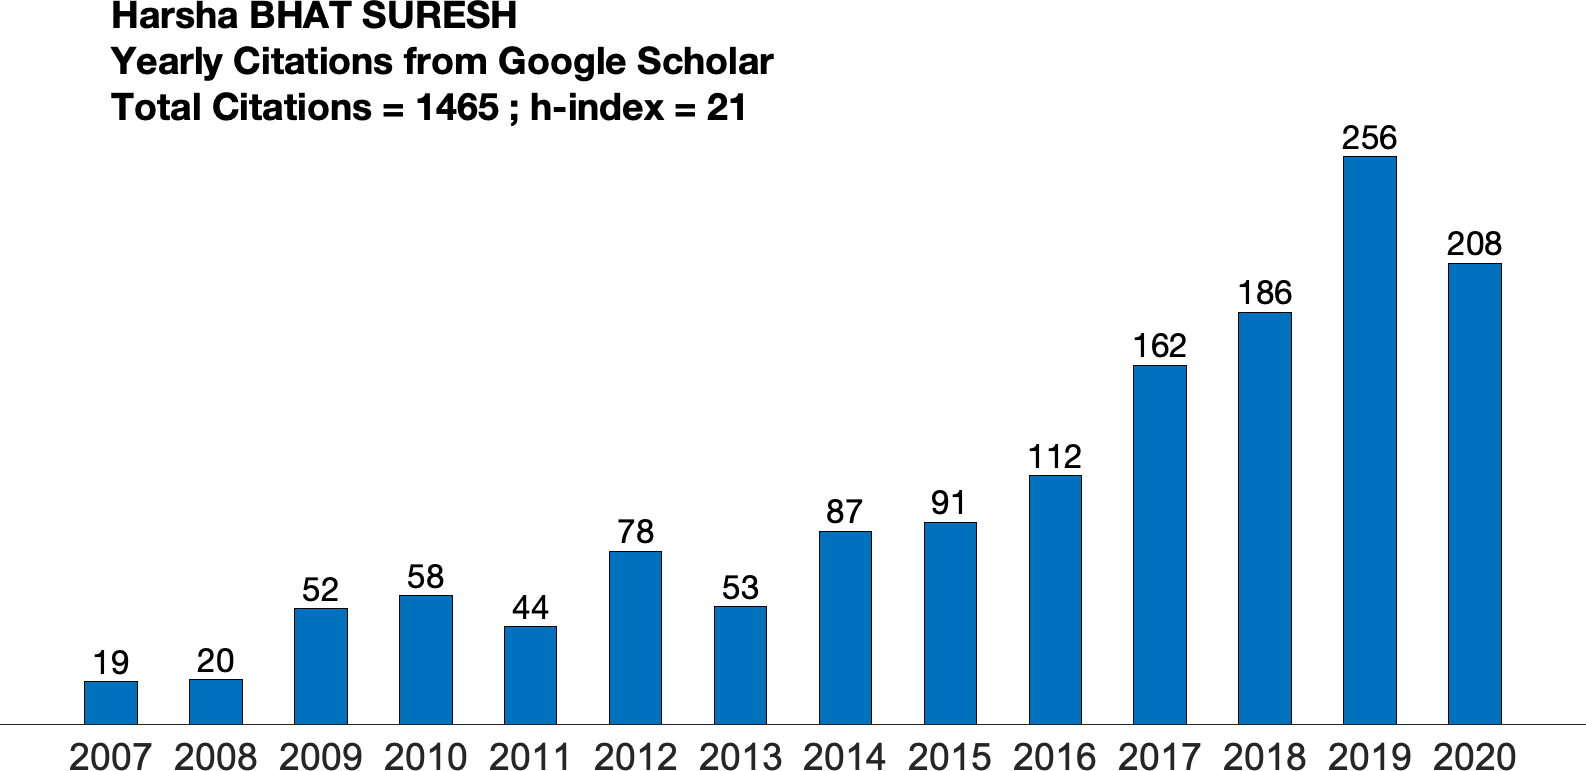
\includegraphics[width=0.60\textwidth]{h.png}
%  \end{center}
% \vspace{-15pt} 
%\end{figure}
%%%%%%%%%%%%%%%%%%%%%%%%%%%%%%%%%%%%%%%%%%%%%%%%%%%%%%%%%%%%%%%%%%%%%%%%
Over 40 publications in peer reviewed international journals including Nature, Nature Communications, Nature Geoscience, Science and Geology. \\[8pt] \href{https://scholar.google.fr/citations?user=ZHskR34AAAAJ&hl=en}{Google Scholar ID: ZHskR34AAAAJ} ~~ \href{https://orcid.org/0000-0003-0361-1854}{ORCID: 0000-0003-0361-1854}\\[-5pt]
\begin{refsegment}
\setlength\bibitemsep{10pt}
\nocite{thomas2020b,romanet2020,marty2020b, jara2020,thomas2020,jeandet2020,amlani2020,jolivet2020,okubo2020, okubo2019,marty2019,aubry2018,klinger2018,cruz2018,thomas2018a,romanet2018,gabuchian2017,thomas2017b,passelegue2017,perol2016,passelegue2016b,mello2016,vallage2015,frank2015,siriki2015,mello2014,passelegue2013,bhat2012,bhat2011a,bhat2010a,biegel2010,mello2010,templeton2010,harris2009,sammis2009,templeton2009,dunham2008a,bhat2007a,bhat2007b,bhat2007c,fliss2005,bhat2004}
\printbibliography[segment=2, title={}, heading=none]
\end{refsegment}
\vspace{10pt}
\vfill\hfill \color{gray}\tiny Last modified \today
%%%%%%%%%%%%%%%%%%%%%%%%%%%%%%%%%%%%%%%%%%%%%%%%%%%%%%%%%%%%%%%%%%%%%%%%%
\end{document}